\begin{samplecase}
{\bf Low energy resonance data for n + ${}^{89}$Y}\newline
TALYS can read in resonance parameters, from various 
possible sources, and call the RECENT code of Red Cullen's PREPRO package, in TALYS included as a subroutine. 
Low energy pointwise resonance cross sections will then be added to channels 
like total, elastic, fission and capture.
\subsubsection{Case a: Resonance input file: Standard}
The input file is

\VerbatimInput{\samples n-Y089-RRR-standard/org/talys.inp}

where {\it n0-2.grid} is the built-in TALYS energy grid for neutrons between 0 and 2 MeV.
\subsubsection{Case b: Resonance input file: Temperature broadening}
The input file is

\VerbatimInput{\samples n-Y089-RRR-temp/org/talys.inp}

\subsubsection{Case c: Resonance input file: Group structure}
The input file is

\VerbatimInput{\samples n-Y089-RRR-group/org/talys.inp}

The results are depicted in Fig. \ref{ngres}. Note the discontinuity between 
the end of the resonance range and the statistical model energy range of TALYS.
Obviously, this needs to be studied case by case.
\end{samplecase}
\begin{figure}
\centering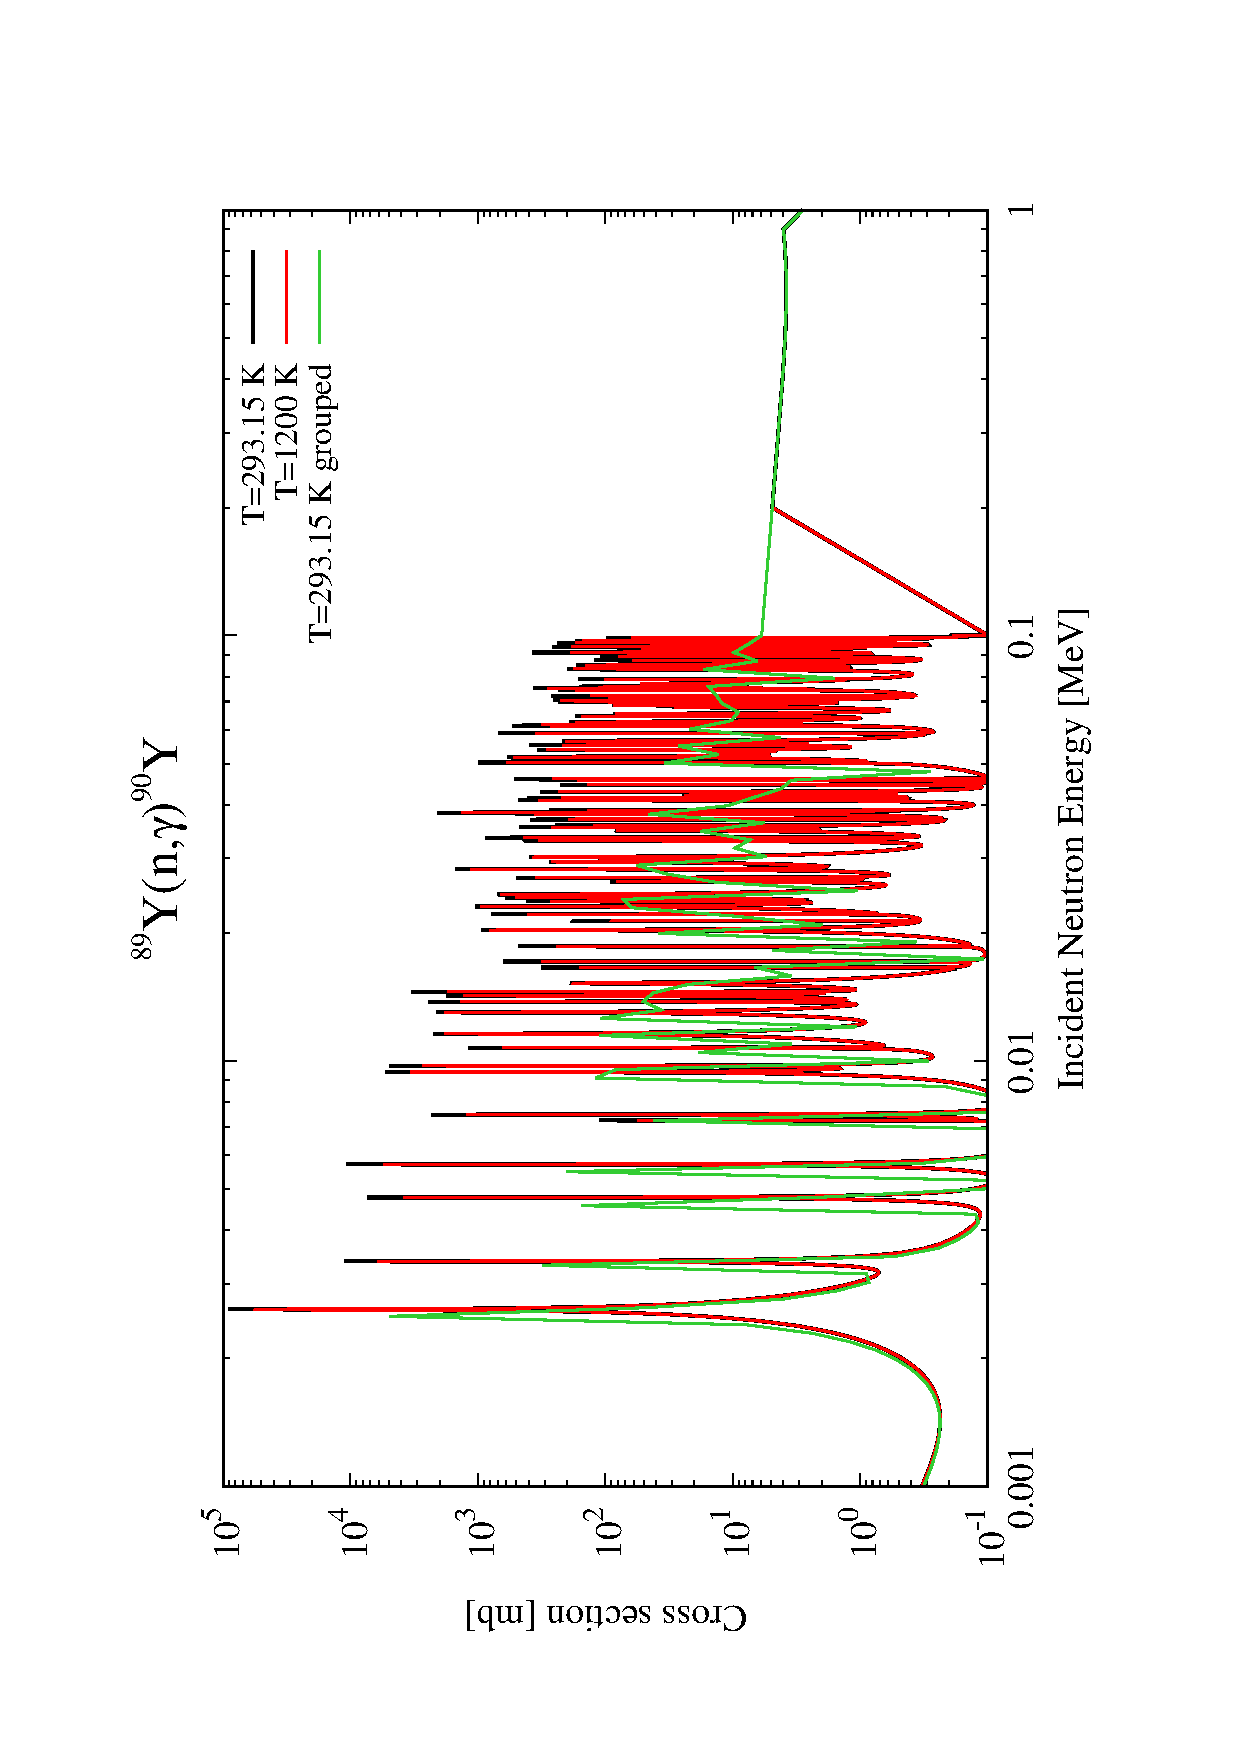
\includegraphics[scale=0.5,angle=270]{n-Y089-RRR}
\caption{${}^{89}$Y(n,$\gamma$) cross section, at 293.15 K, 1200 K, and grouped.}
\label{ngres}
\end{figure}
